\documentclass[10pt]{IEEEtran}
% correct bad hyphenation here
%\hyphenation{op-tical net-works semi-conduc-tor}

\usepackage{algorithm, algpseudocode, amsmath, cite, graphicx, multirow, url}

\makeatletter
\newcommand{\removelatexerror}{\let\@latex@error\@gobble}
\makeatother

\begin{document}

\title{Tag Recommendations in StackOverflow}
\author{Logan~Short, Christopher~Wong, and~David~Zeng}% <-this % stops a space
\markboth{CS 224W Final Project, Autumn 2014}{}
\maketitle

\begin{abstract}
Abstract goes here.
\end{abstract}

\section{Introduction}

\IEEEPARstart{S}{tackOverflow} is a piece of horse shit.

\section{Prior Work}

Before analyzing existing implementations of tag recommendation systems, we found abundant relevant information regarding the growth and properties of groups and communities in large social networks. In \cite{2}, McAuley and Leskovec propose an algorithm to automatically discover social circles by analyzing the similarities among user profiles in data drawn from the social networking sites Facebook, Google+, and Twitter. Using the idea that nodes are well connected within a circle, the algorithm finds the best parameters to determine which edges should exist in an ego network. In \cite{3}, Backstrom et al. analyze the evolution of communities in social networks over time. The authors use a decision tree model to classify communities as fast- or slow-growing and show that connectedness of the community within and to those outside of the community plays a huge role in growth rate.

In \cite{1}, Xia et al. propose an automatic tag recommendation algorithm \textit{TagCombine}. There are three components of \textit{TagCombine}, each of which tries to assign the best tags to untagged objects: (1) multi-label ranking component, which predicts tags using a multi-label learning algorithm, (2) similarity based ranking component, which uses similar objects to recommend tags, and (3) tag-term based ranking component, which analyzes the historical affinity of tags to certain words in order to suggest tags. The recommendation algorithm methodically computes various weighted sums of the three components to attempt to find the best overall model. A $recall@k$ score is then calculated for each prediction model from stratified $10$-fold cross validation. (The $recall@k$ metric is discussed more in Section $4$.) \textit{TagCombine} does significantly better than all other cited models.

In \cite{5}, Wang et al. propose a tag recommendation system dubbed \textit{EnTagRec}. The proposed \textit{EnTagRec} computes tag probability scores using two separate methods, Bayesian Inference and Frequentist Inference, and then takes a weighted sum of the probability scores. Bayesian Inference relies on a post’s textual data to compute the probability that a given tag is associated with the post. \textit{EnTagRec} formulates posts into a bag-of-words model and then trains a Labeled Latent Dirichlet Allocation model which is used to compute tag probability scores for a post. The Frequentist Inference approach infers a set of tags after some preprocessing of a post. Once this set is computed, \textit{EnTagRec} applies spreading activation to a tag network constructed by examining the co-occurrence rate of tags on the site. Experimental results show that \textit{EnTagRec} performs significantly better than \textit{TagCombine} from \cite{1} on Stack Overflow, Ask Ubuntu, and Ask Different datasets, but yields only comparable results on Freecode datasets.

In \cite{1}, Xia et al. propose a recommendation system that relates the textual features of posts to tags with reasonably good results. However, one weakeness of \textit{TagCombine} is that it fails to look at the network structure of software information sites. Posts on sites like Stack Overflow are ultimately connected to each other through an underlying network structure where users and tags that appear on multiple posts represent connections between said posts. In fact, tags exist in order to group similar posts and create an organized structure that allows for more convenient and logical browsing of posts. Thus, it makes sense that knowledge of the network’s structure could be used to enhance a tag recommendation system. In \cite{5}, Wang et al. provide evidence that such an approach could yield significant improvement in tag recommendation results. In \cite{5}, the basic \textit{TagCombine} model proposed in \cite{1} is enhanced into a model that uses not only textual analysis of posts, but also network analysis of the tags themselves. Although results improved, the use of network structure is very limited, and further incorporation of network structure could potentially lead to more accurate tag recommendations.

One weakness in both \cite{1} and \cite{5} is that they both only address tag recommendations during question creation time. That is, tag recommendations need to be made with just the text from the initial post. Discussion generated over time by the post is not factored into the features for the tag recommendation system. However, tagging a post is not an action limited to post creation time. Users may add additional tags to posts later on based on the discussion. In the context of a social network, this is similar to the notion of users joining new communities: posts can acquire new tags over time. This train of thought brings us back to the discussion of clustering of nodes in networks. In \cite{2}, McAuley and Leskovec discuss a method for automatically detecting ``circles'' in networks of users based on similarities in user profiles. A natural extension of this method would be to detect posts associated with common tags based on the similarities in features of the posts or to find circles of tags or users that could allow for accurate detection of possible associated tags using a given tag. Both situations are realistic for clustering tags, users, or posts on software information sites.

\section{Data and Network Analysis}

\subsection{Data Collection}

\subsection{Tag Synonyms}

We refer to two tags as tag synonyms if their names are different but they refer to the same concept, such as \texttt{.net-3.5} and \texttt{.net-framework-3.5}. Tag synonyms are a direct result of a question poster being given full discretion to assign tags to his or her post and to arbitrarily create new tags. Since the pruning of tag synonyms is currently done manually by various contributors to the site, there are still many synonyms groups throughout the site. Figure~\ref{fig:syn} is a screenshot of the \textit{Tag Synonyms} page of StackOverflow taken on December 9, and we can see that the maintenance of this list varies consistency.\\

\begin{figure}[h]
  \centering
    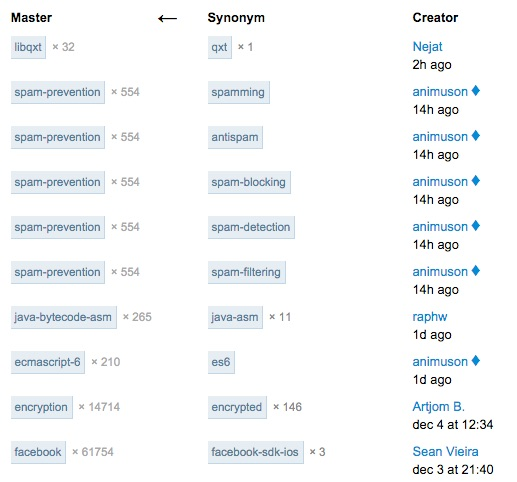
\includegraphics[width=3.2in]{tagsynonyms_so.jpg}
  \caption{Screenshot of \textit{Tag Synonyms} page.}
  \label{fig:syn}
\end{figure}

To be able to test the effects of tag synonyms on our tag recommendation model, we prepared a separate tag list derived from our initial set of $437$ after manually pruning for tag synonyms. Since these tags are among the more popular tags in the StackOverflow community, we were only able to reduce this new set to a size of $428$ after coalescing tags such as \texttt{report} and \texttt{reporting}. We expect this pruned list of tags to moderately, but not drastically, improve our results.

\subsection{Network Features}

\subsubsection{Network Based on Post Similarity}

\subsubsection{Network Based on User Interaction}

\subsubsection{Bipartite Graph between Users and Tags}

\section{Algorithm and Results}

\subsection{Original TagCombine Components}

To begin, using the procedures described in \cite{1}, we implemented the three major components of the \textit{TagCombine} algorithm to establish a baseline for the performance of our tag recommendation system. By reproducing a working implementation of \textit{TagCombine}, we were able analyze the effect of our improvements on tag recommendation accuracy.

As alluded to earlier, \cite{1} introduces the concept of the $recall@k$ metric for measuring the success of a tag recommendation model, where $k$ is a tunable parameter that determines how many tags the model recommends for each object. Intuitively, over $n$ objects, the $recall@k$ metric measures the average success rate in predicting correct tags for each object, where a ``correct'' tag is simply a tag that has been used to label that particular object by an actual user. Let $R_i$ be the set of tags recommended for object $i$ (so, $|R_i| = k$), and let $T_i$ be the actual set of tags used to label object $i$. Then, the formula for $recall@k$ is:

\[recall@k = \frac{1}{n}\sum\limits_{i=1}^{n}\frac{|R_i \cap T_i|}{|T_i|}.\]

\subsubsection{Multilabel Learning Algorithm}

\subsubsection{Similarity Based Ranking Component}

\subsubsection{Tag-term Based Ranking Component}

\subsection{New Network Based Ranking Component}

\subsubsection{Modification to Similarity Component}

\subsection{NetTagCombine Algorithm}

In our proposed tag recommendation system, \textit{NetTagCombine}, we add our new Network-Based Ranking Component, alongside the other components of \textit{TagCombine}. Building upon the equation for \textit{TagCombine} given in \cite{1}, for all tags $t$ with respect to some post $p$, our new \textit{NetTagCombine} score can be given by
\begin{align*}
NetTagCombine_p(t) =\ &\alpha \times MultiLabel_p(t) +\\
&\beta \times SimRank_p(t) +\\
&\gamma \times TagTerm_p(t) +\\
&\delta \times Network_p(t)
\end{align*}
where $\alpha,\beta,\gamma,\delta \in [0,1]$ represent the different weights of the components. Here, we have added the term of $\delta \times Network_p(t)$ to represent our new fourth component that uses the underlying network structure. To adjust for this fourth component, here is the pseudocode for \textit{NetTagCombine}:


\begin{algorithm*}
  \caption{\textit{NetTagCombine} algorithm}\label{ntc}
  \begin{algorithmic}[1]
    \State $\alpha, \beta, \gamma, \delta \gets 0$
    \For{\textbf{all }posts $p$}
      \For{\textbf{all }tags $t \in TAGS$}
        \State Compute \textit{MultiLabel}$_p(t)$, \textit{SimRank}$_p(t)$, \textit{TagTerm}$_p(t)$, and \textit{Network$_p(t)$}
      \EndFor
    \EndFor
    \For{\textbf{all }$\alpha$ from $0$ to $1$, every time increment by $0.2$}
      \For{\textbf{all }$\beta$ from $0$ to $1$, every time increment by $0.2$}
        \For{\textbf{all }$\gamma$ from $0$ to $1$, every time increment by $0.2$}
          \For{\textbf{all }$\delta$ from $0$ to $1$, every time increment by $0.2$}
            \State Compute \textit{NetTagCombine}$_p(t)$ for all tags $t$ on posts $p$
            \State Evaluate effectiveness of $(\alpha,\beta,\gamma,\delta)$ from $recall@k$ scores
          \EndFor
        \EndFor
      \EndFor
    \EndFor\\
    \Return Best $(\alpha,\beta,\gamma,\delta)$\;
  \end{algorithmic}
\end{algorithm*}

\subsection{Results}

\section{Conclusion}

\subsection{Future Work}

\begin{thebibliography}{1}
\bibitem{1} X. Xia, D. Lo, X. Wang, B. Zhou. Tag Recommendation in Software Information Sites. MSR, 2013.
\bibitem{2} J. McAuley, J. Leskovec. Discovering Social Circles In Ego Networks. ACM TKDD, 2014.
\bibitem{3} L. Backstrom, D. Huttenlocher, J. Kleinberg, X. Lan. Group Formation in Large Social Networks: Membership, Growth, and Evolution. KDD, 2006.
\bibitem{4} J. Leskovec, K. Lang, A. Dasgupta, M. Mahoney. Statistical Properties of Community Structure in Large Social and Information Networks. WWW, 2008.
\bibitem{5} S. Wang, D. Lo, B. Vasilescu, A. Serebrenik. EnTagRec: An Enhanced Tag Recommendation System for Software Information Sites. ICSME, 2014.
\bibitem{6} Stack Exchange Data Dump (September 26, 2014). Retrieved 2 November 2014. https://archive.org/details/stackexchange.
\end{thebibliography}

%\balancecolumns

\end{document}
